\documentclass[10pt,a4paper]{article}
\usepackage[margin=22mm]{geometry}
\usepackage[T1]{fontenc}
\usepackage{lmodern,microtype,booktabs,tabularx,xcolor,enumitem,amsmath}
\usepackage{tikz}
\usetikzlibrary{arrows.meta,positioning,calc,fit}
\usepackage[colorlinks=true,linkcolor=blue!50!black]{hyperref}
\setlist{itemsep=1pt,topsep=3pt}
\newcommand{\code}[1]{\texttt{#1}}
\newcommand{\meas}{\textsuperscript{M}}
\newcommand{\est}{\textsuperscript{E}}
% ---- measured totals used in the text ----
\newcommand{\regcore}{334}
\newcommand{\regcg}{334}
\newcommand{\regsoc}{336}
\newcommand{\reglat}{114}
\newcommand{\regtotal}{1{,}118}
\newcommand{\rtllines}{3{,}515}
\newcommand{\ngsoccells}{53{,}794}
\newcommand{\ngsocarea}{0.090 mm$^2$}
\newcommand{\ngsocflops}{6{,}987}
\newcommand{\skysoccells}{54{,}572}
\newcommand{\skysocarea}{0.420 mm$^2$}
\newcommand{\skysocflops}{6{,}987}
\newcommand{\skysocpath}{13.9 ns}
\title{\textbf{Gust N1 v1.0}\\[2pt]\large A two-core, Linux-capable processor system grown from the Gust microcontroller\\Architecture and test report (spec v1)}
\author{Designed for Allan \quad$\cdot$\quad 16 November 2026}
\date{}
\begin{document}
\maketitle
\vspace{-8mm}
\noindent\fbox{\parbox{0.97\linewidth}{\small
\textbf{How to read the numbers.} \meas{} marks a value measured in this project (simulation or synthesis).
\est{} marks an estimate, with the derivation given next to it. Everything unmarked is a design decision.
Nothing in this document was measured on silicon or on an FPGA.}}

\section{Summary}
Gust N1 v1.0 is a complete processor \emph{system} in synthesizable Verilog: two Gust-based cores, each with a
memory-management unit and an instruction cache, sharing one memory bus, with the timer and interrupt
controllers an operating system needs and a port for external RAM of any size.

It has every hardware feature that RV32 Linux requires of a processor. Linux itself has \textbf{not} been
booted on it; section~\ref{sec:linux} lists what that still takes.

\begin{center}\small
\begin{tabular}{@{}ll@{}}
\toprule
Instruction set & RV32IMAC, Zicsr, Zifencei, Zba, Zbb, Zbs, Zcb (\code{misa} = \code{0x40141107})\\
Privilege and memory & M, S and U modes; Sv32 paging; 8-entry TLB with hardware page-table walker\\
Cores & 2 (parameter \code{NCORES}); one fast-multiply core and one small-multiply core\\
Tests\meas & \regtotal{} test runs, all pass (section~\ref{sec:verif})\\
Speed per MHz\meas & 2.87 CoreMark/MHz with 1-cycle RAM; 2.02 with RAM that needs 2 wait cycles\\
Core size, 130 nm\meas & 22{,}399 cells, 0.173 mm$^2$ of cells, 11.4 ns logic path\\
Core size, 45 nm\meas & 23{,}585 cells, 0.038 mm$^2$ of cells, 2.57 ns logic path\\
40 nm target\est & about 0.045 mm$^2$ per core placed; 150--200 MHz for the system (section~\ref{sec:40nm})\\
\bottomrule
\end{tabular}
\end{center}

\section{What changed from N1 v0.1 to v1.0}
N1 v0.1 was a single core with privilege modes and paging. Version 1.0 adds the rest of the list.

\begin{center}\small
\begin{tabularx}{\linewidth}{@{}lXl@{}}
\toprule
Added in v1.0 & Why Linux needs it & File\\
\midrule
Atomic instructions (A) & Locks and counters shared between cores; the kernel will not build without them & \code{gust\_core.v}, \code{gust\_decode.v}\\
Core-local interruptor & The timer tick and the ``wake the other core'' interrupt & \code{n1\_clint.v}\\
Interrupt controller & Routes device interrupts to a core, in M or S mode & \code{n1\_plic.v}\\
Shared memory bus & Lets several cores use one RAM; keeps atomics atomic & \code{n1\_membus.v}\\
Instruction cache & Makes slow external RAM usable; keeps the cores off each other's bus time & \code{n1\_icache.v}\\
System top level & Cores, controllers, UART and the external RAM port & \code{n1\_soc.v}\\
\bottomrule
\end{tabularx}
\end{center}

\section{Architecture: one bus, stacked filters}\label{sec:arch}
The Gust core is a three-stage pipeline with two bus ports (instructions and data). N1 keeps that core and
its pipeline. Every feature a computer chip needs is added as a block that has the Gust bus on \emph{both}
sides, so blocks stack like filters on a pipe and the core does not know they are there.

\begin{center}
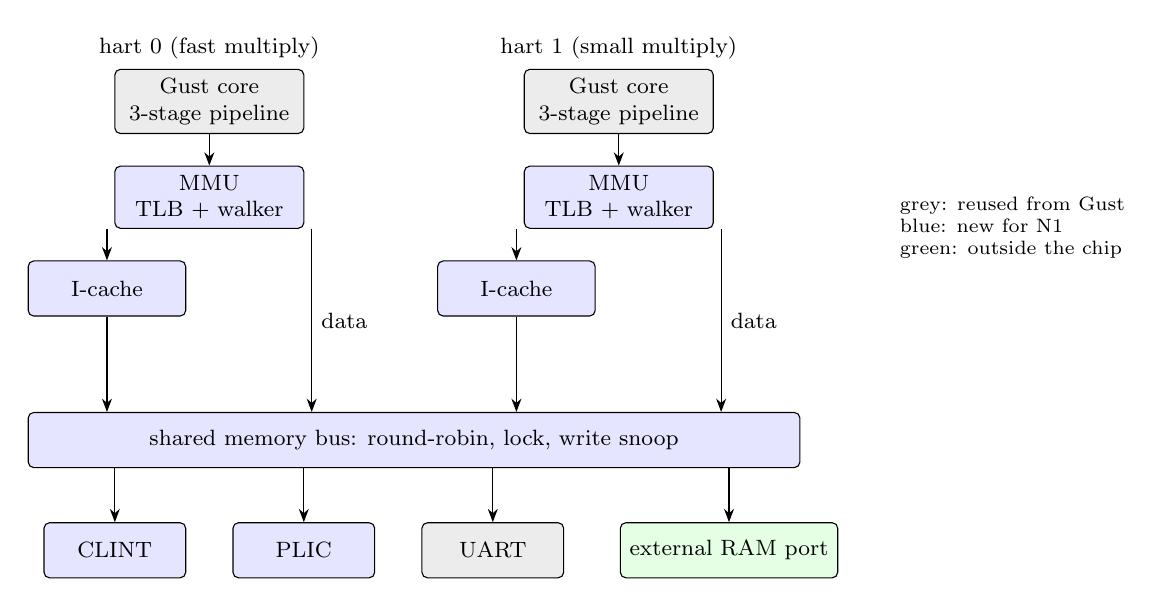
\begin{tikzpicture}[font=\footnotesize,>=Stealth,
  b/.style={draw,rounded corners=2pt,minimum height=7mm,minimum width=24mm,align=center},
  n/.style={b,fill=blue!10}, r/.style={b,fill=gray!15}]
\foreach \h/\x/\t in {0/0/{hart 0 (fast multiply)},1/5.2/{hart 1 (small multiply)}} {
  \node[r] (c\h) at (\x,0) {Gust core\\3-stage pipeline};
  \node[n,below=4mm of c\h] (m\h) {MMU\\TLB + walker};
  \node[n,below=4mm of m\h,xshift=-13mm,minimum width=20mm] (i\h) {I-cache};
  \draw[->] (c\h) -- (m\h);
  \draw[->] (m\h.south) ++(-13mm,0) -- (i\h.north);
  \coordinate (d\h) at ($(m\h.south)+(13mm,0)$);
  \node[above=0mm of c\h] {\t};
}
\node[n,minimum width=98mm] (bus) at (2.6,-4.3) {shared memory bus: round-robin, lock, write snoop};
\foreach \h in {0,1} { \draw[->] (i\h.south) -- (i\h.south|-bus.north); \draw[->] (d\h) -- (d\h|-bus.north) node[midway,right]{data}; }
\node[n,minimum width=18mm] (cl) at (-1.2,-5.7) {CLINT};
\node[n,minimum width=18mm] (pl) at (1.2,-5.7) {PLIC};
\node[r,minimum width=18mm] (ua) at (3.6,-5.7) {UART};
\node[b,minimum width=26mm,fill=green!10] (ram) at (6.6,-5.7) {external RAM port};
\foreach \k in {cl,pl,ua,ram} \draw[->] (\k.north|-bus.south) -- (\k.north);
\node[font=\scriptsize,align=left] at (10.2,-1.6) {grey: reused from Gust\\blue: new for N1\\green: outside the chip};
\end{tikzpicture}
\end{center}

\noindent Three consequences of this structure:
\begin{itemize}
\item \textbf{Reuse.} Six Gust files are used unchanged and five are modified; the pipeline stages are the
same ones that were tested in Gust (section~\ref{sec:reuse}).
\item \textbf{Faults look like bus errors.} A page fault comes back from the MMU on the same wire as a bus
error, with one extra wire that says ``this was a page fault''. The core's existing trap logic handles both.
\item \textbf{The price.} A translated address must pass through the TLB before it reaches the bus in the
same cycle. That lengthens the core's critical path from 8.0 ns (Gust) to 11.4 ns\meas{} on 130 nm, and
the shared bus lengthens the system's path further (section~\ref{sec:40nm}). Section~\ref{sec:faster}
describes the fixes, which are not built.
\end{itemize}

\section{The new blocks}
\subsection{Atomic instructions}
\textbf{Read-modify-write (\code{amoadd.w} and the other eight).} The execute stage runs a short sequence:
read the word with the bus \emph{locked}, compute, write, unlock. While the lock is held the shared bus
gives no other core a turn, so no other core can change the word in between. The read is marked ``write
intended'' so the MMU checks write permission \emph{before} anything happens; a fault therefore never
leaves a half-done operation.

\textbf{Load-reserved and store-conditional (\code{lr.w}, \code{sc.w}).} Each core has one reservation: a
valid bit and a \emph{physical} word address. \code{lr.w} sets it. The shared bus shows every write to
every core (the ``snoop''); a write by anyone to the reserved word clears the reservation. \code{sc.w}
writes only if the reservation is still valid, and always clears it. Traps also clear it.

\emph{Example.} Two cores both run \code{lr.w} on a counter, add one, and run \code{sc.w}. Whichever
\code{sc.w} reaches the bus first writes; that write is snooped by the other core and cancels its
reservation, so its \code{sc.w} fails and the software loop retries. The two-core test does exactly this
600 times and checks that the counter ends at 600.

\subsection{Instruction cache}
One per core, direct mapped, 64 lines of 4 words (1 KiB of instructions, about 9{,}700 memory bits with
tags\meas). A hit answers one cycle after the request, exactly like on-chip RAM in Gust. A miss fetches
the 4-word line from the shared bus. The cache sits after the MMU, so it is indexed by physical address
and does not need flushing when page tables change. \code{fence.i} flushes it.

The cache is read-only, so two cores never hold conflicting copies of data. It does not watch other
cores' writes: code that is modified must be followed by \code{fence.i} on each core that will run it,
which is what the RISC-V rules already require and what Linux does.

\subsection{Shared memory bus}
Four masters (instruction and data port of each core), one grant per cycle, round-robin so no core
starves. It adds the lock used by atomics and the write snoop used by reservations. A request that is
waiting for the RAM to accept it stays selected until accepted. This rule was added after the test bench
caught the bus switching masters in the middle of a wait.

\subsection{Timer and interrupt controllers}
\begin{center}\small
\begin{tabular}{@{}lll@{}}
\toprule
Block & Address & Contents\\
\midrule
CLINT & \code{0x0200\_0000} & software interrupt bit per core (\code{+4h}); \code{mtimecmp} per core (\code{0x4000+8h}); \code{mtime} (\code{0xBFF8})\\
PLIC & \code{0x0C00\_0000} & 7 sources, 3-bit priority, 2 contexts per core (M and S), claim and complete\\
UART & \code{0x1000\_0000} & the Gust UART; PLIC source 1\\
RAM & \code{0x8000\_0000} & external port; anything not listed above goes here\\
\bottomrule
\end{tabular}
\end{center}
The register layout of the CLINT and PLIC follows the usual RISC-V layout, so existing firmware and
Linux drivers for them should apply. The UART is Gust's own and is not 16550-compatible.

\subsection{RAM}
The system has no RAM inside. It has a 32-bit external memory port with a ready/valid handshake, so the
RAM may take any number of cycles to answer. The test bench attaches 512 KiB; the address space allows
up to 2 GiB at \code{0x8000\_0000}. A real board would put an SDRAM or PSRAM controller on this port.
That controller is not part of this release.

\subsection{An asymmetric pair}
Both cores are the same Verilog. One parameter gives hart 0 the single-cycle multiplier (2{,}546 cells,
about 11\% of a core\meas) and hart 1 the 32-cycle multiplier. This shows that mixed cores cost no
extra design work in this structure. It is a small difference, not a ``big'' and a ``little'' core in the
phone-chip sense. \code{ASYM=0} builds two identical cores.

\section{How Gust was reused}\label{sec:reuse}
\begin{center}\small
\begin{tabularx}{\linewidth}{@{}lX@{}}
\toprule
Unchanged from Gust v1.0 & compressed-instruction expander, ALU, multiplier/divider, register file, clock gate, UART\\
Modified & definitions, fetch (page-fault wire), decoder (privileged and atomic instructions), core (privilege checks, atomic sequence), CSR file (rewritten for M/S/U)\\
New for N1 & MMU, core wrapper, I-cache, shared bus, CLINT, PLIC, system top\\
\bottomrule
\end{tabularx}
\end{center}
The 18 files total \rtllines{} lines of Verilog\meas.

\section{Verification}\label{sec:verif}
All tests run in the Icarus Verilog simulator under cocotb. Each test is run twice: once with the
memory answering immediately and once with random wait cycles on every access.

\begin{center}\small
\begin{tabularx}{\linewidth}{@{}Xrr@{}}
\toprule
Target\meas & Runs & Pass\\
\midrule
Single core: 166 official RISC-V tests (user, machine, supervisor, atomics; 60 of them running under paging) + privilege and paging test & \regcore & \regcore\\
Same, with register-file clock gating on & \regcg & \regcg\\
Two-core system: all of the above on hart 0 through cache and shared bus, + two-core test & \regsoc & \regsoc\\
Two-core system with slow RAM (2 wait cycles), subset & \reglat & \reglat\\
\midrule
Total & \regtotal & \regtotal\\
\bottomrule
\end{tabularx}
\end{center}

\textbf{The two-core test} (\code{tb/sw/n1\_smp.c}) starts both cores and checks: 600 increments each by
\code{amoadd.w}, by an \code{lr.w}/\code{sc.w} loop, and by a plain counter guarded by an
\code{amoswap.w} spinlock; an inter-core interrupt in each direction; a timer interrupt on each core;
PLIC priority, enable, threshold, claim and complete, in M and S contexts; and that both cores compute
the same products while hart 1 takes more than twice as long to multiply.

\textbf{Checking the checks.} A test that cannot fail proves nothing, so three deliberate bugs were put
into the design, one at a time, and removed again:
\begin{center}\small
\begin{tabular}{@{}ll@{}}
\toprule
Deliberate bug & Result\meas\\
\midrule
Reservations are never cancelled by another core's write & two-core test fails (lost updates)\\
\code{sc.w} always succeeds & two-core test fails (lost updates)\\
Bus lock is ignored & two-core test hangs and is stopped by the time limit\\
\bottomrule
\end{tabular}
\end{center}

\textbf{A failure worth recording.} The first full run of the two-core system failed one test. The
single-core privilege test did not park hart 1, so both cores ran it at once and shared its counters. The
test's start-up code was corrected and everything was run again; the hardware was not changed.

\textbf{What is not covered.} The official tests run on hart 0 only. Hart 1 is exercised only by the
two-core test. There is no random instruction testing, no formal proof, and no long two-core stress run.
An operating system boot is the usual next test and normally finds bugs that these tests miss.

\section{Performance}\label{sec:perf}
CoreMark, 10 iterations, GCC \code{-O2}, one core, run to completion in Verilator on the full system\meas.
``Wait cycles'' are extra cycles the external RAM takes on every access.

\begin{center}
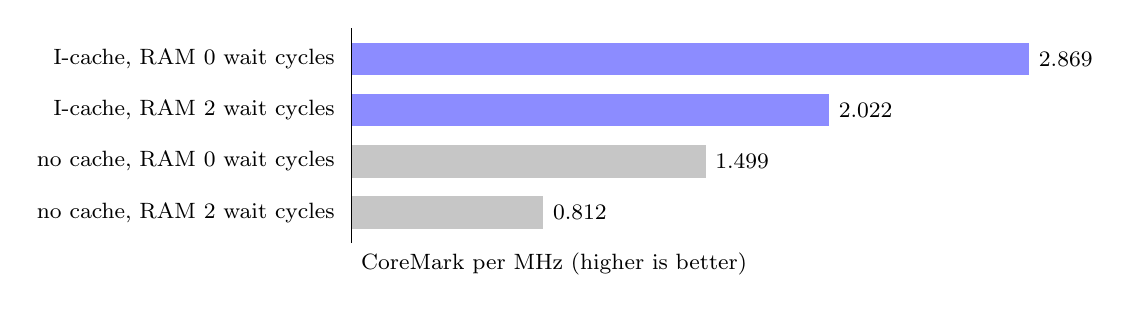
\begin{tikzpicture}[font=\footnotesize,x=30mm,y=6.5mm]
\foreach \y/\v/\l/\c in {3/2.869/{I-cache, RAM 0 wait cycles}/blue!45,2/2.022/{I-cache, RAM 2 wait cycles}/blue!45,
                         1/1.499/{no cache, RAM 0 wait cycles}/gray!45,0/0.812/{no cache, RAM 2 wait cycles}/gray!45} {
  \fill[\c] (0,\y-0.32) rectangle (\v,\y+0.32);
  \node[anchor=east] at (-0.03,\y) {\l};
  \node[anchor=west] at (\v,\y) {\v};
}
\draw (0,-0.6) -- (0,3.6);
\node[anchor=west] at (0,-1.0) {CoreMark per MHz (higher is better)};
\end{tikzpicture}
\end{center}

\noindent What the four bars say:
\begin{itemize}
\item With fast RAM the full system reaches 2.87, against 2.93 for the Gust microcontroller with on-chip
RAM. The MMU, cache and shared bus cost about 2\% per MHz.
\item The instruction cache is worth 1.9 times with fast RAM and 2.5 times with slow RAM. The no-cache
configuration needs a register between core and bus, which costs it one cycle per fetch.
\item With slow RAM the system drops from 2.87 to 2.02. That loss is on the data side, which has no
cache. A data cache is the largest remaining speed gain (section~\ref{sec:faster}).
\end{itemize}
Two-core throughput was not measured.

\section{Size, speed and the 40 nm question}\label{sec:40nm}
\subsection{Measured synthesis}
Yosys with a delay-oriented ABC script, typical corner. ``Logic path'' is the longest path through gates
only: no wires, no clock tree, no placement. Real chips are slower than this number.

\begin{center}\small
\begin{tabular}{@{}lrrrl@{}}
\toprule
Block\meas & Cells & Cell area & Flip-flops & Logic path\\
\midrule
\multicolumn{5}{@{}l}{\emph{SkyWater 130 nm (hd)}}\\
Gust v1.0 core (for reference) & 16{,}315 & 0.122 mm$^2$ & 1{,}756 & 8.0 ns\\
N1 v0.1 core & 20{,}817 & 0.162 mm$^2$ & 2{,}423 & 11.2 ns\\
N1 v1.0 core (core + MMU, with atomics) & 22{,}399 & 0.173 mm$^2$ & 2{,}521 & 11.4 ns\\
Shared bus, 4 masters & 462 & 0.003 mm$^2$ & 9 & --\\
CLINT, 2 cores & 1{,}440 & 0.014 mm$^2$ & 244 & --\\
PLIC, 2 cores & 874 & 0.007 mm$^2$ & 83 & --\\
I-cache control (without its memory) & about 430 & 0.006 mm$^2$ & about 130 & --\\
Two-core system, caches cut to 4 lines & \skysoccells & \skysocarea & \skysocflops & \skysocpath\\
\midrule
\multicolumn{5}{@{}l}{\emph{Nangate 45 nm open cell library}}\\
N1 v1.0 core & 23{,}585 & 0.038 mm$^2$ & 2{,}526 & 2.57 ns\\
Two-core system, caches cut to 4 lines & \ngsoccells & \ngsocarea & \ngsocflops & 3.55 ns\\
\bottomrule
\end{tabular}
\end{center}
The system rows were synthesized with 4-line caches, so the full cache memories (2 $\times$ 9{,}700 bits) are not in them. Built from
flip-flops they would be larger than both cores together, so a real chip would use small memory macros.
The cache control figures are derived from two synthesis runs at different sizes.

\subsection{From 45 nm to 40 nm}
No open 40 nm library exists, so 40 nm cannot be measured here. The Nangate 45 nm library is the closest
open one, and it is a \emph{predictive} library, not a foundry's. The 40 nm figures below are estimates
built on it.

\begin{itemize}
\item \textbf{Area\est.} 40 nm is a 0.9 linear shrink of 45 nm, so area scales by about $0.9^2 = 0.81$.
Core cells: $0.038 \times 0.81 \approx 0.031$ mm$^2$. Placed at 70\% density:
$0.031 / 0.7 \approx 0.045$ mm$^2$ per core. Two cores, controllers and two 1 KiB caches: roughly
0.12--0.15 mm$^2$ of core area, before pads. At this size the pad ring, not the logic, sets the die size.
\item \textbf{Clock\est.} The clock is set by the whole system, not by one core. The system's logic
path is 3.55 ns\meas{} on 45 nm, longer than the core's 2.57 ns, because a data address goes through the TLB,
the bus arbiter and the address decoder in one cycle. 3.55 ns means 280 MHz with ideal wires. Wires, clock
skew and setup margin typically add 30--40\%, giving about 5 ns or 200 MHz. Foundry low-power 40 nm cells
are slower than the predictive library, so the working estimate is \textbf{150--200 MHz}. The same
reasoning on 130 nm (13.9 ns\meas) gives about 50 MHz.
\item \textbf{Throughput\est.} $2.87 \times 150$ to $2.87 \times 200$ gives roughly 430--570 CoreMark
per core with caches hitting. That is the class of soft-core Linux systems and early ARM9 Linux boards.
A Raspberry Pi 5 is more than ten times faster per core and has four of them; N1 is not in that class
and this structure will not get there.
\end{itemize}
Power was not estimated; that needs a placed design and switching activity.

\section{What is unusual here, and what is not}
You asked for a less standard approach that still is Gust. This is where N1 differs from the common
way of building a small Linux core, and how new each point really is.

\begin{center}\small
\begin{tabularx}{\linewidth}{@{}lXX@{}}
\toprule
Choice & Common practice & N1\\
\midrule
Where the MMU lives & TLB lookup is a pipeline step; the pipeline is designed around it & A bus filter outside an unchanged microcontroller pipeline\\
Page faults & Separate exception path from the TLB & Returned as a bus error with one flag wire\\
Atomics on several cores & Cache-line ownership in a coherent data cache & Bus lock and bus write snoop; no data cache to keep coherent\\
Taken branches & Predictor tables, one or more lost cycles on a miss & Inherited from Gust: direction and target decoded in fetch, no lost cycle when predicted taken\\
Mixed cores & Two separate core designs & One design, one parameter\\
\bottomrule
\end{tabularx}
\end{center}
None of these is a research result. Each idea exists somewhere in older or smaller designs. What is
particular to N1 is using all of them to turn a microcontroller core into a multi-core Linux-class system
by adding blocks around it. The cost is clock speed (the TLB in the address path) and data-side speed
(no data cache).

\section{The faster N1 (designed, not built)}\label{sec:faster}
These are the next changes, in order of expected gain. None is implemented or tested.

\begin{enumerate}
\item \textbf{Data cache as another bus filter.} Write-through, so RAM is always up to date and the
existing lock and snoop keep working: a snooped write from another core invalidates the matching line.
Its request register also cuts the long TLB-to-arbiter path of section~\ref{sec:40nm}.
Expected to recover most of the gap between 2.02 and 2.87 CoreMark/MHz with slow RAM\est.
\item \textbf{Early translation from the base register.} Most addresses are ``register plus small
offset'', and the offset rarely changes the page. Look up the TLB with the base register's page number
at the start of the cycle, in parallel with the adder, and check afterwards that the page did not change;
if it did, take one extra cycle. This removes the TLB from the critical path and should bring the logic
path back near Gust's 8.0 ns on 130 nm\est, about 40\% more clock speed.
\item \textbf{Predecoded instruction cache.} Store Gust's fetch-stage predecode bits (length, branch,
target) in the cache line, so fetch does not recompute them on every hit.
\item \textbf{Larger TLB with address-space IDs,} so a context switch does not empty the TLB.
\item \textbf{More cores.} \code{NCORES} is a parameter and the bus is generic, but only 2 was tested,
and a single shared bus stops scaling at about four cores.
\end{enumerate}

\section{From here to a Linux boot}\label{sec:linux}
The processor features are present. The remaining work is software and one memory controller. None
of it has been tried.

\begin{enumerate}
\item \textbf{Boot firmware.} OpenSBI for RV32, with a small console driver for the Gust UART. It runs in
M mode, starts hart 1, and provides the timer service to the kernel.
\item \textbf{Device tree} describing two \code{rv32imac} cores with Sv32, the CLINT, the PLIC, the UART
and the RAM.
\item \textbf{Kernel and user programs.} A 32-bit RISC-V kernel configured without floating point, and a
Buildroot root file system built for \code{rv32imac}. Mainstream distributions do not support 32-bit
RISC-V, so the user programs must be built this way.
\item \textbf{RAM.} At least 32 MiB in the simulation model, and an SDRAM or PSRAM controller for a board.
\item \textbf{A fast simulator run.} A boot is several hundred million cycles or more\est, so it must run
in Verilator, not Icarus. The Verilator build of the system exists (\code{tb/verilator}).
\end{enumerate}

\section{Known limitations}
\begin{itemize}
\item Linux has not been booted. No operating system of any kind has run on N1.
\item No data cache; every load and store goes to the external RAM.
\item No floating-point unit and no physical memory protection (PMP).
\item The TLB has 8 entries shared by instructions and data, without address-space IDs.
\item The Gust debug module (JTAG) is not connected in the N1 system.
\item Hart 1 is tested only by the two-core test; only \code{NCORES=2} was tested.
\item The no-cache option (\code{ICACHE=0}) exists for the comparison in section~\ref{sec:perf} and was run only with CoreMark.
\item Timing figures are logic-only synthesis. No place and route, no sign-off timing, no power figures.
\item The 45 nm library is predictive and the 40 nm figures are estimates.
\item Not run on an FPGA. The Verilator lint still reports width warnings in \code{n1\_plic.v} and
\code{n1\_clint.v}; they were reviewed and are harmless size extensions.
\item The UART is not 16550-compatible, so Linux needs a console through the boot firmware or a small driver.
\end{itemize}

\section{Files and how to run}
\begin{center}\small
\begin{tabularx}{\linewidth}{@{}lX@{}}
\toprule
\code{rtl/} & 18 Verilog files; \code{n1\_soc.v} is the top level\\
\code{tb/} & \code{make prepare} builds the tests; \code{make core\_isa core\_isa\_cg soc\_isa soc\_isa\_lat2} runs them\\
\code{tb/verilator/} & fast build of the system; used for CoreMark\\
\code{syn/} & \code{synth.tcl} for Yosys; 130 nm and 45 nm settings are in its header\\
\code{docs/} & this document\\
\bottomrule
\end{tabularx}
\end{center}
Tools used: Icarus Verilog, cocotb 2, Verilator 5, Yosys 0.33, the RISC-V GCC toolchain and the official
\code{riscv-tests} suite.
\end{document}
